\section{Query Processing}

We are now at the top two layers of Figure \ref{fig:arch}.

See Figure \ref{fig:overview} for a general overview of all the steps when processing a query. The left side is how it has always been (precompiled modules) and nowadays there is the new trend to directly generate code to execute a query even more efficiently since it allows for more specific cases. This distinction is not that important.

\begin{figure}[h]
	\centering
	\includegraphics[scale=0.4]{images/3-overview.PNG}
	\caption{Steps of query processing.}
	\label{fig:overview}
\end{figure}



\subsection{Introduction}

To process / parse a query sent from a client (DB application), it is first allocated to a process / thread through a DB engine interface while validating it, checking access control (permissions) and matching it with the query cache. Then, for each uncached query, a query plan (operator tree) is created (possibly rewriting and optimizing the query) and executed while buffers are read from the DB buffer cache or from disk. Finally, the results are sent back to the client.

A DB engine is commonly a shared environment with many users running queries concurrently while the engine itself runs its own maintenance procedures. A DB engine is similar to an OS since it has to schedule, orchestrate and mediate access to shared resources.

In a commercial setting, DBs are used programmatically meaning that queries generated by user interfaces are created by application programs. The use of views and query templates affects query processing.


\paragraph{Caching}
In a DB system, it is very likely to receive the same query multiple times and sometimes even in a short time frame. The best way to speed up execution is to reuse results from a previous execution (parsing, optimization, query itself, (intermediate) results\footnote{Query results can be cached in the engine itself or outside of it (intermediate layer, client-side caching, etc.).}, etc.) - everything can be cached! This also works well for data that does not change much (e.g. BLOBS / large data items). As always, consistency problems have to be dealt with.


\paragraph{Memory Structures}
Memory needs to be managed carefully since we have many different things running at the same time and shared vs. local memory has to be differentiated. It is common to divide it into regions each with a single purpose.

\paragraph{Cursor}
A pointer to a data structure (table, view, result, etc.) used to navigate the structure - similar to the iterator concept in programming languages. Space needs to be allocated to manage its state (opened, closed, accessed, etc.). When a table is processed, a cursor moves from tuple to tuple. Also used when delivering results to clients - instead of returning a possibly huge table, the cursor to it is returned.





\subsection{Execution Models}

When processing an SQL query, it is parsed into a tree of operators which is the basis for the execution model (see Figure \ref{fig:tree}). The leaves are the tables involved in the query and the root is the final result. Typically, each operator has at most two input from the lower layers (join). Operators can read input / output results one tuple at a time or as a whole - some are even blocking (all operations need to be completed until result can be issued). Each query and each subtree is its own table.

\begin{figure}[h]
	\centering
	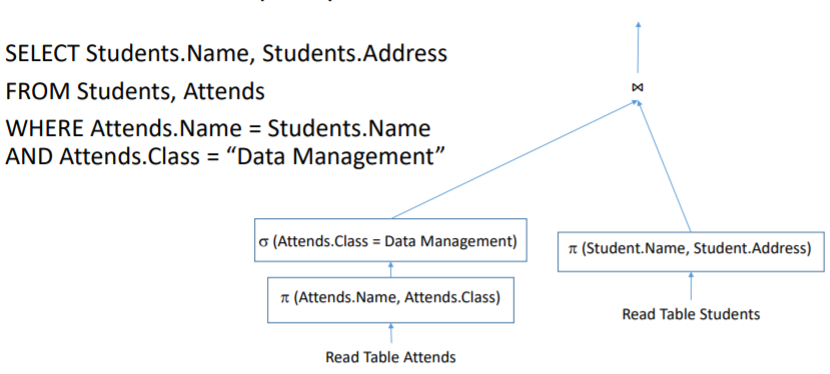
\includegraphics[scale=0.6]{images/3-tree.PNG}
	\caption{Query plan of an example SQL query.}
	\label{fig:tree}
\end{figure}

\paragraph{Pull Mode}
An operator obtains data through a function call to a lower operator (control moves top-down) - data is obtained whenever it is needed. Good for disk-based systems and whenever the data doesn't fit in memory.

\paragraph{Push Mode}
A lower operator sends its result up as soon as it completes processing a tuple / buffer / vector. Higher operators receive results and potentially have to buffer them if they're not ready yet to process them. Can be more efficient than pull mode (hardware / CPU exploitation) but it's more difficult to implement (buffer, synchronization, etc.) - similar to event-based programming. See example in Figure \ref{fig:push}.

\begin{figure}[h]
	\centering
	\includegraphics[scale=0.5]{images/3-push.PNG}
	\caption{Push mode example.}
	\label{fig:push}
\end{figure}


\subsubsection{Single Machine Execution Models}


\paragraph{Iterator Model (or Volcano / Pipeline)}
Tuples = data traverse the tree from leaves to the root. Operators iterate over those tuples to process them by using the interface \texttt{Next()}. The execution (control) is top-down (the \texttt{Next()} call initiated at the top trickles down until it can be executed). Once both tables (left and then right) are filled, the nested for-loop is executed. Widely used in disk-based systems and works for all workloads. See Figure \ref{fig:iterator}.

\textbf{Pros:} Generic interface for all operators (great information hiding). Iterators are easy to implement. Supports buffer management strategies. No overhead in terms of main memory. Supports pipelining, parallelism and distribution (with special iterators).

\textbf{Cons:} High overhead of method calls (context switches) and poor instruction cache locality (jumping down and up in the tree calling different functions).

\begin{figure}[h]
	\centering
	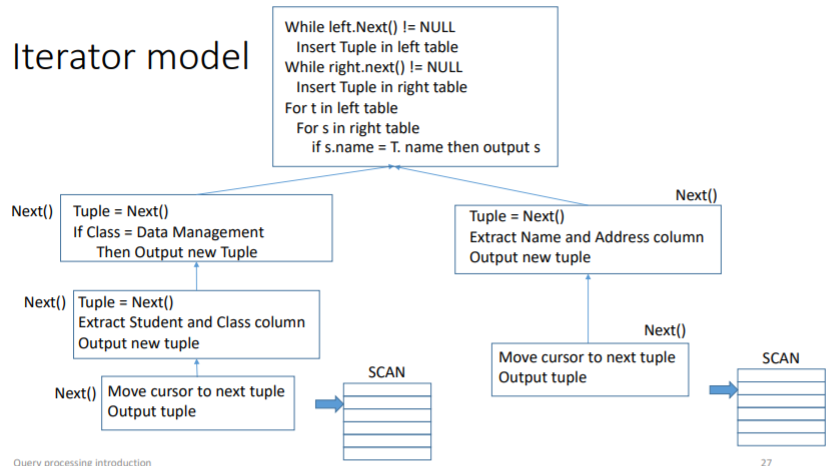
\includegraphics[scale=0.7]{images/3-iterator.PNG}
	\caption{Iterator model of example SQL query (typo: "Name" instead of "Student" in left block).}
	\label{fig:iterator}
\end{figure}

\paragraph{Materialization Model}
Similar to the iterator model but instead of outputting one tuple at a time, each operator outputs its result in a single buffer (each operator is called only once). Much less method calls - less overhead than previous model. Works well in OLTP (queries / transactions process small amounts of data resulting in small buffers that are passed around) - assuming data fits in memory. Not suitable for OLAP since data being passed around can be very large. See Figure \ref{fig:material}.

\begin{figure}[h]
	\centering
	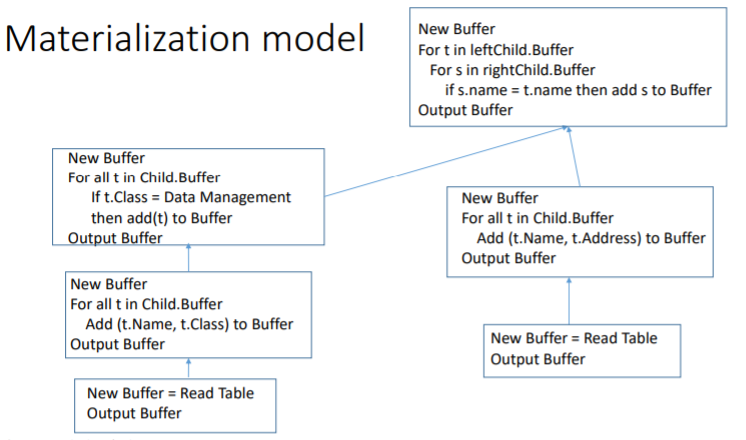
\includegraphics[scale=0.7]{images/3-material.PNG}
	\caption{Materialization model of example SQL query.}
	\label{fig:material}
\end{figure}

\paragraph{Vectorized / Batch Model}
Exploits SIMD / AVX (and column-store) by combining the iterator and materialization model. Data is iterated over with \texttt{Next()} which returns a set of tuples (e.g. entire column) instead of a single one resp. a full buffer. This works best for OLAP systems. %TODO example?

\begin{figure}[h]
	\centering
	\includegraphics[scale=0.7]{images/3-excomp.PNG}
	\caption{Comparison of execution models.}
	\label{fig:excomp}
\end{figure}



\subsubsection{Parallel Processing Execution Models}

To parallelize a plan or distribute it across several machines, the above models can simply be extended with an \texttt{EXCHANGE} operator. The operator only moves data from one place (e.g. machine) to another - it does not modify data. See Figure \ref{fig:exchange}.

\begin{figure}[h]
	\centering
	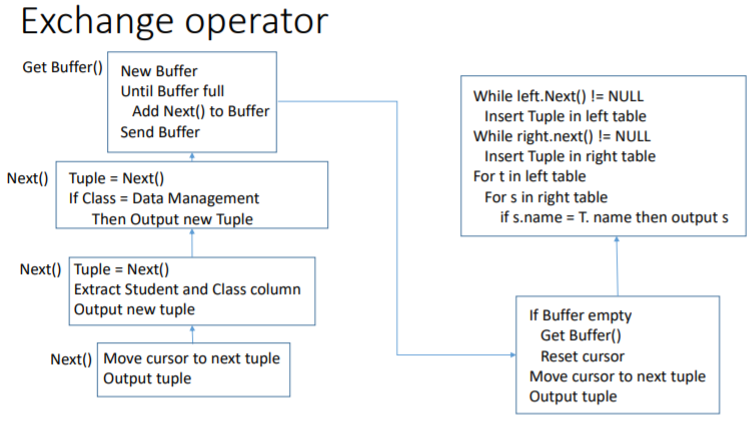
\includegraphics[scale=0.7]{images/3-exchange.PNG}
	\caption{One way to implement an exchange operator (as a driver) shown with example SQL query.}
	\label{fig:exchange}
\end{figure}


\subsection{Query Optimization}

Since SQL is declarative, a DB engine has many options to translate a query into an executable program. After generating possible execution plans for a query, the best one has to be chosen (based on rules or based on estimated cost). A plan is influenced by the access methods for each table (leaves of the query tree), i.e. available indices, predicates, clustered tables (same extent), type of operator implementation, i.e. join implementation, sorted data, and the shape and form of the query tree.

\paragraph{View}
The result set of a stored query on the data (virtual table). A view can be queried just like any other persistent database collection object. Changes applied to the relevant underlying data are perpetuated. A view can me materialized into an actual table and added to the schema (usually done for common operations over the schema). Mainly used to implement logical data independence (create schema different from original one) and access control (access view instead of base tables).





\subsubsection{Query Rewriting}

After a query has been parsed, it is often rewritten into an equivalent query based on the DB schema and on some heuristics. The rewritten query is then used as input for the query optimization process. 

Rewriting can remove operations to make the query more efficient, can give the optimizer more freedom to operate, can make the query's intent more explicit and can map it to actual base tables and views as needed / for efficiency reasons.


\paragraph{View Expansion}
Each view reference appearing in the FROM clause is rewritten to the actual definition of the view (fetched from the catalog manager). Applied recursively until query is fully expressed over base tables.

\paragraph{Constant Arithmetic Evaluation}
Things like $r.x < 10 + 2 + r.y$ are rewritten to $r.x < 12 + r.y$.

\paragraph{Logical Predicate Rewriting}
Apply logical rewrites to predicates and constants in the WHERE clause. Just apply simple Boolean logic. This also includes predicate augmentation based on transitive closures to include more predicates for the optimizer to choose from (e.g. A=B, B=C - also add A=C; A=B, B$>$100 - also add A$>$100; etc.).

\paragraph{Semantic Optimization}
Integrity constraints are stored in the catalog and can be used to rewrite queries. Examples: redundant join elimination cased on foreign key constraints or removing the DISTINCT clause for primary keys. 

\paragraph{Query Unnesting and Normalization}
A query can include multiple nested query which can be flattened. For some queries, there exists an equivalent canonical form that is easier to process.

\paragraph{Examples}
Examples in Figures \ref{fig:transormation}, \ref{fig:aug1} and \ref{fig:aug2}.

\begin{figure}[h]
	\centering
	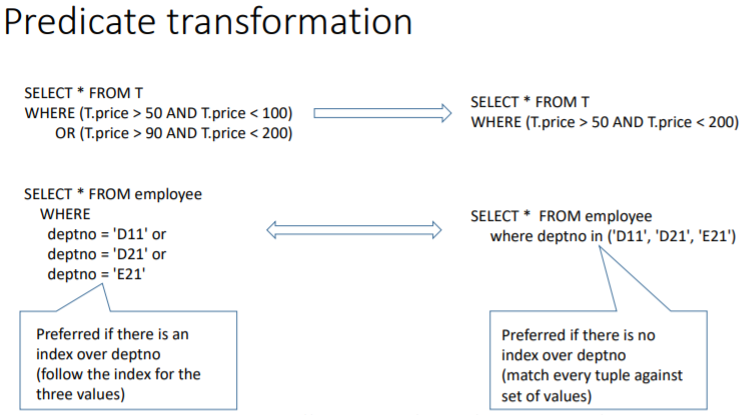
\includegraphics[scale=0.5]{images/3-transformation.PNG}
	\caption{Predicate transformation example.}
	\label{fig:transormation}
\end{figure}

\begin{figure}[h]
	\centering
	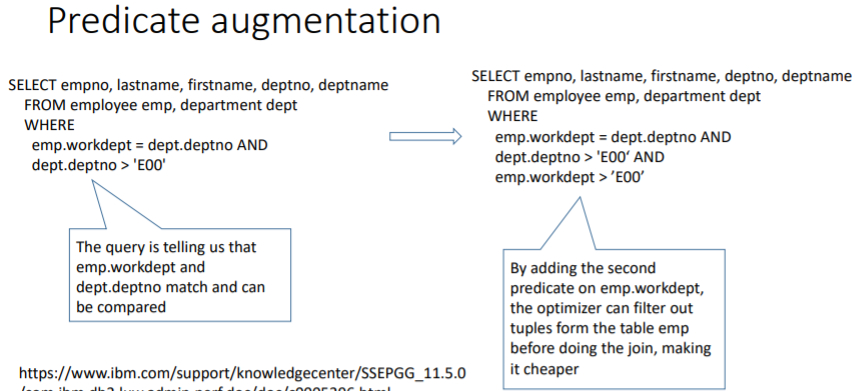
\includegraphics[scale=0.5]{images/3-aug1.PNG}
	\caption{Predicate augmentation example 1.}
	\label{fig:aug1}
\end{figure}

\begin{figure}[h]
	\centering
	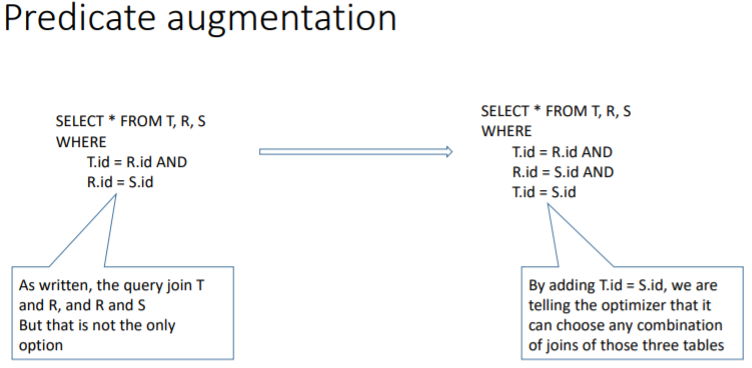
\includegraphics[scale=0.5]{images/3-aug2.PNG}
	\caption{Predicate augmentation example 2.}
	\label{fig:aug2}
\end{figure}

%TODO more examples from slides

\paragraph{Equivalence Rules}
With relational algebra, we can prove equivalence over queries (equivalence rules). This enables query transformations with the guarantee that the results stay the same. See extra sheet for all the rules.











\subsubsection{Cost Based Optimization}

To choose the best query plan out of multiple equivalent ones for a query, we might rely on its estimated cost based on many types of information. We need to factor in the access method for each table that is at the leaf level of the query tree (how are the tables stored, is there an index, etc.), what implementation to choose for the operators (type of join, sorting, etc.) and the shape of the query tree (order of operations, etc.).

Example: find all possible ways to access leaf tables and estimate the cost and selectivity - pick the best one. Then, generate all possible orders (e.g. join orders) and estimate the cost for each. Pick the best.

In contrast, a rule-based optimizer does not look at statistics or the contents of the tables - it uses rules only (transformation rules, method rankings, schema info, etc.). Rules are based on experience.

\paragraph{Statistics}
Statistics that are constantly collected on tables, indices, buffers and the system itself can be an information source for query optimization (which plan and which operator implementation). We have:

\begin{itemize}
    \item \textbf{Table Statistics:} Number of rows / blocks / etc., average row length, etc.
    \item \textbf{Column Statistics:} Number of distinct values / nulls / etc. (helps to estimate selectivity of a predicate or to decide on join order), data distribution (histogram), etc.
    \item \textbf{Extended Statistics:} Index statistics, number of leaf blocks, levels, clustering factor, etc.
    \item \textbf{System Statistics:} I/O performance and utilization, CPU performance and utilization, etc.
\end{itemize}

For example, when joining two tables, the smaller one should be the outer loop. For a hash join, the smaller table is usually the one the hash index is built over (easy to maintain) while the bigger one is used for probing (only loop).


\paragraph{Histogram}
Histograms can help estimate the cardinality of different kinds of operations.

\textbf{Equi-Width:} Each bucket of the histogram has the same width (interval length).

\textbf{Equi-Height:} Each bucket of the histogram has the same height (number of data points). It is likely that the width of each bucket varies. Very suited to estimate the result of joins.

\textbf{Singleton / Frequency:} Histogram plots the frequency of every distinct item in a table. Useful to compute selectivity of a query. Chosen if the number of distinct items (NDV) is smaller than the number of buckets of the histogram.

\textbf{Top N Frequency:} Only record the frequencies of the n most frequent values while all other values are represented in the same column.

\textbf{Hybrid:} Histogram types can be combined. E.g. equi-width and most frequent.

\paragraph{Zone Map}
For every block of a table, keep the max and min values for some or all columns. Before reading a block, read those values to check if predicate is in the range - if not, don't read the block. Other statistics can be kept in a zone map and in some cases it can replace an index.

\paragraph{Cardinality}
There are different definitions of cardinality when talking about a DBMS:
\begin{itemize}
    \item \textbf{Attribute:} Number of distinct values of that attribute. Estimated using statistics.
    \item \textbf{Table:} Number of tuples in that table.
    \item \textbf{Operator:} Number of tuples to be processed to get result = input. Depends on input table, operator and access method.
    \item \textbf{Predicate:} How many tuples match predicate.
\end{itemize}

\paragraph{Selectivity}
How much data an operator will produce. Typically expressed as a fraction over data in the table (1: all, 0: none). Related to attribute cardinality.
\begin{itemize}
    \item Equality predicate on key = one tuple.
    \item Equality predicate on non-key = in case of uniform data approximated by number of tuples / number of distinct values. If skewed, use histogram.
    \item Range predicate: use histogram or assume uniform distribution.
    \item Negation predicate = 1 - predicate.
    \item Independent distribution of values for each predicate: conjunction just multiply, disjunction add selectivities minus selectivity of intersection (selectivity of conjunction).
    \item Predicates over correlated attributes: complex. Use hisogram.
\end{itemize}



\subsubsection{Operators}

See Figure \ref{fig:relalg} for an overview of relational algebra operators and the techniques used to implement them. See \href{https://www.javatpoint.com/selection-operation-in-query-processing}{here} for a good reference on how to implement relational algebra operations.

\begin{figure}[h]
	\centering
	\includegraphics[scale=0.6]{images/3-relalg.PNG}
	\caption{Relational algebra operators and their implementation.}
	\label{fig:relalg}
\end{figure}

\paragraph{Selection}
A selection is performed by scanning files using a search algorithm that locates the data we want to access.
\begin{itemize}
    \item \textbf{Linear Search:} Always works but usually slow, just seek the file and scan its pages (extra seeks needed if they're not stored in a contiguous order). For each record scanned, check if the selection applies.
    \item \textbf{Using Indexes (Access Paths):} Primary vs. secondary, equality on key vs. non-key, or comparison. Keep I/O in mind in secondary index.
\end{itemize}

\paragraph{Join Algorithms}
There are many different ways to perform a join.
\begin{itemize}
    \item \textbf{Nested-Loop:} A loop nested in another, for each record check if join predicate holds. Worst case complexity is number of records of outer loop times number of records in inner loop. Basically a cross product. $N*M$
    \item \textbf{Block Nested-Loop:} Load large chunks of outer relation into main memory and for each chunk scan other relation.
    \item \textbf{Index Join:} For each record in inner loop, query index on outer relation if it contains the inner relation record.
    \item \textbf{Hash Join:} Same as index join but instead of accessing the index, access the hash table. $N+M$
    \item \textbf{Sort-Merge Join:} Sort both tables on join attribute, linear scan for join. Might require an external sort if tables cannot be sorted in memory. $N*logN + M*logM$
\end{itemize}

%TODO cost stuff.... uuugghghhhghhgjghjghjghg


%TODO Rest of slides, has hjoin external join




\paragraph{Two-Phase External Sort}
We have N input pages and a buffer with M slots. In the first phase, we create runs of size M that are sorted in memory and written back to disk. In the second phase, a priority heap is used to merge the individually sorted runs. If M is smaller than the square root of N, multiple merge phases are necessary (multi-way merge).

Multi-way merge cost: B buffer pages and N pages to sort - cost $= 2N * (1 + log_{B-1} \frac{N}{B})$ (rounded up)

%TODO external hash, grace hash, partitioned hash, multi pass radix partitioning (end of operators)










\subsection{Reading Assignments}

\subsubsection{Sort vs. Hash Revisited}

\subsubsection{Query Optimization}

\subsubsection{The State of the Art in Distributed Query Processing}








\subsection{Exercises}

\subsubsection{Query Processing}

\paragraph{Engine Caching}
\begin{itemize}
    \item False: predicate matching is used to check for identical previous queries in library cache in most systems. Too expensive, especially in concurrent environments.
    \item True: Simple string matching is used to check for identical previous queries in library cache in most system. Very easy.
    \item False: Cache lookups for queries are cheap due to fast memory and thus complex query equivalence checks for query matching are always performed. Too complex.
    \item True: OLAP applications benefit from result caches. 
\end{itemize}

\paragraph{Client-Server Systems:}
\begin{itemize}
    \item True: In C-S systems, administration of only server systems is necessary.
    \item False: C-S systems usually lower cost than P2P.
    \item False: C-S security is enforced by both sides.
    \item True: Executing queries on client side can exploit additional computational resources.
\end{itemize}

\paragraph{Middle-Tier Caching:}
\begin{itemize}
    \item False: Applications are more difficult to write for the architectures with intermediate layer caching compared to client caching.
    \item True: middle-tier adds to scalability, caching service scales better than client caching, consistency only between intermediate and server.
\end{itemize}

\paragraph{Query vs. data shipping:}
Investment: number of non-result pages to transfer from server to client with client doing the query execution. Benefit: number of result pages if server executes query. If query is repeated, the benefit might outweigh the investment after a certain number of repetitions.

E.g. I = 120, B = 20 - 6 iterations.



\subsubsection{Query Rewriting}

\subsubsection{Query Optimization}

\subsubsection{Cost-Based Optimizer}

\subsubsection{Query Operators}
